\documentclass[1p]{elsarticle_modified}
%\bibliographystyle{elsarticle-num}

%\usepackage[colorlinks]{hyperref}
%\usepackage{abbrmath_seonhwa} %\Abb, \Ascr, \Acal ,\Abf, \Afrak
\usepackage{amsfonts}
\usepackage{amssymb}
\usepackage{amsmath}
\usepackage{amsthm}
\usepackage{scalefnt}
\usepackage{amsbsy}
\usepackage{kotex}
\usepackage{caption}
\usepackage{subfig}
\usepackage{color}
\usepackage{graphicx}
\usepackage{xcolor} %% white, black, red, green, blue, cyan, magenta, yellow
\usepackage{float}
\usepackage{setspace}
\usepackage{hyperref}

\usepackage{tikz}
\usetikzlibrary{arrows}

\usepackage{multirow}
\usepackage{array} % fixed length table
\usepackage{hhline}

%%%%%%%%%%%%%%%%%%%%%
\makeatletter
\renewcommand*\env@matrix[1][\arraystretch]{%
	\edef\arraystretch{#1}%
	\hskip -\arraycolsep
	\let\@ifnextchar\new@ifnextchar
	\array{*\c@MaxMatrixCols c}}
\makeatother %https://tex.stackexchange.com/questions/14071/how-can-i-increase-the-line-spacing-in-a-matrix
%%%%%%%%%%%%%%%

\usepackage[normalem]{ulem}

\newcommand{\msout}[1]{\ifmmode\text{\sout{\ensuremath{#1}}}\else\sout{#1}\fi}
%SOURCE: \msout is \stkout macro in https://tex.stackexchange.com/questions/20609/strikeout-in-math-mode

\newcommand{\cancel}[1]{
	\ifmmode
	{\color{red}\msout{#1}}
	\else
	{\color{red}\sout{#1}}
	\fi
}

\newcommand{\add}[1]{
	{\color{blue}\uwave{#1}}
}

\newcommand{\replace}[2]{
	\ifmmode
	{\color{red}\msout{#1}}{\color{blue}\uwave{#2}}
	\else
	{\color{red}\sout{#1}}{\color{blue}\uwave{#2}}
	\fi
}

\newcommand{\Sol}{\mathcal{S}} %segment
\newcommand{\D}{D} %diagram
\newcommand{\A}{\mathcal{A}} %arc


%%%%%%%%%%%%%%%%%%%%%%%%%%%%%5 test

\def\sl{\operatorname{\textup{SL}}(2,\Cbb)}
\def\psl{\operatorname{\textup{PSL}}(2,\Cbb)}
\def\quan{\mkern 1mu \triangleright \mkern 1mu}

\theoremstyle{definition}
\newtheorem{thm}{Theorem}[section]
\newtheorem{prop}[thm]{Proposition}
\newtheorem{lem}[thm]{Lemma}
\newtheorem{ques}[thm]{Question}
\newtheorem{cor}[thm]{Corollary}
\newtheorem{defn}[thm]{Definition}
\newtheorem{exam}[thm]{Example}
\newtheorem{rmk}[thm]{Remark}
\newtheorem{alg}[thm]{Algorithm}

\newcommand{\I}{\sqrt{-1}}
\begin{document}

%\begin{frontmatter}
%
%\title{Boundary parabolic representations of knots up to 8 crossings}
%
%%% Group authors per affiliation:
%\author{Yunhi Cho} 
%\address{Department of Mathematics, University of Seoul, Seoul, Korea}
%\ead{yhcho@uos.ac.kr}
%
%
%\author{Seonhwa Kim} %\fnref{s_kim}}
%\address{Center for Geometry and Physics, Institute for Basic Science, Pohang, 37673, Korea}
%\ead{ryeona17@ibs.re.kr}
%
%\author{Hyuk Kim}
%\address{Department of Mathematical Sciences, Seoul National University, Seoul 08826, Korea}
%\ead{hyukkim@snu.ac.kr}
%
%\author{Seokbeom Yoon}
%\address{Department of Mathematical Sciences, Seoul National University, Seoul, 08826,  Korea}
%\ead{sbyoon15@snu.ac.kr}
%
%\begin{abstract}
%We find all boundary parabolic representation of knots up to 8 crossings.
%
%\end{abstract}
%\begin{keyword}
%    \MSC[2010] 57M25 
%\end{keyword}
%
%\end{frontmatter}

%\linenumbers
%\tableofcontents
%
\newcommand\colored[1]{\textcolor{white}{\rule[-0.35ex]{0.8em}{1.4ex}}\kern-0.8em\color{red} #1}%
%\newcommand\colored[1]{\textcolor{white}{ #1}\kern-2.17ex	\textcolor{white}{ #1}\kern-1.81ex	\textcolor{white}{ #1}\kern-2.15ex\color{red}#1	}

{\Large $\underline{11n_{6}~(K11n_{6})}$}

\setlength{\tabcolsep}{10pt}
\renewcommand{\arraystretch}{1.6}
\vspace{1cm}\begin{tabular}{m{100pt}>{\centering\arraybackslash}m{274pt}}
\multirow{5}{120pt}{
	\centering
	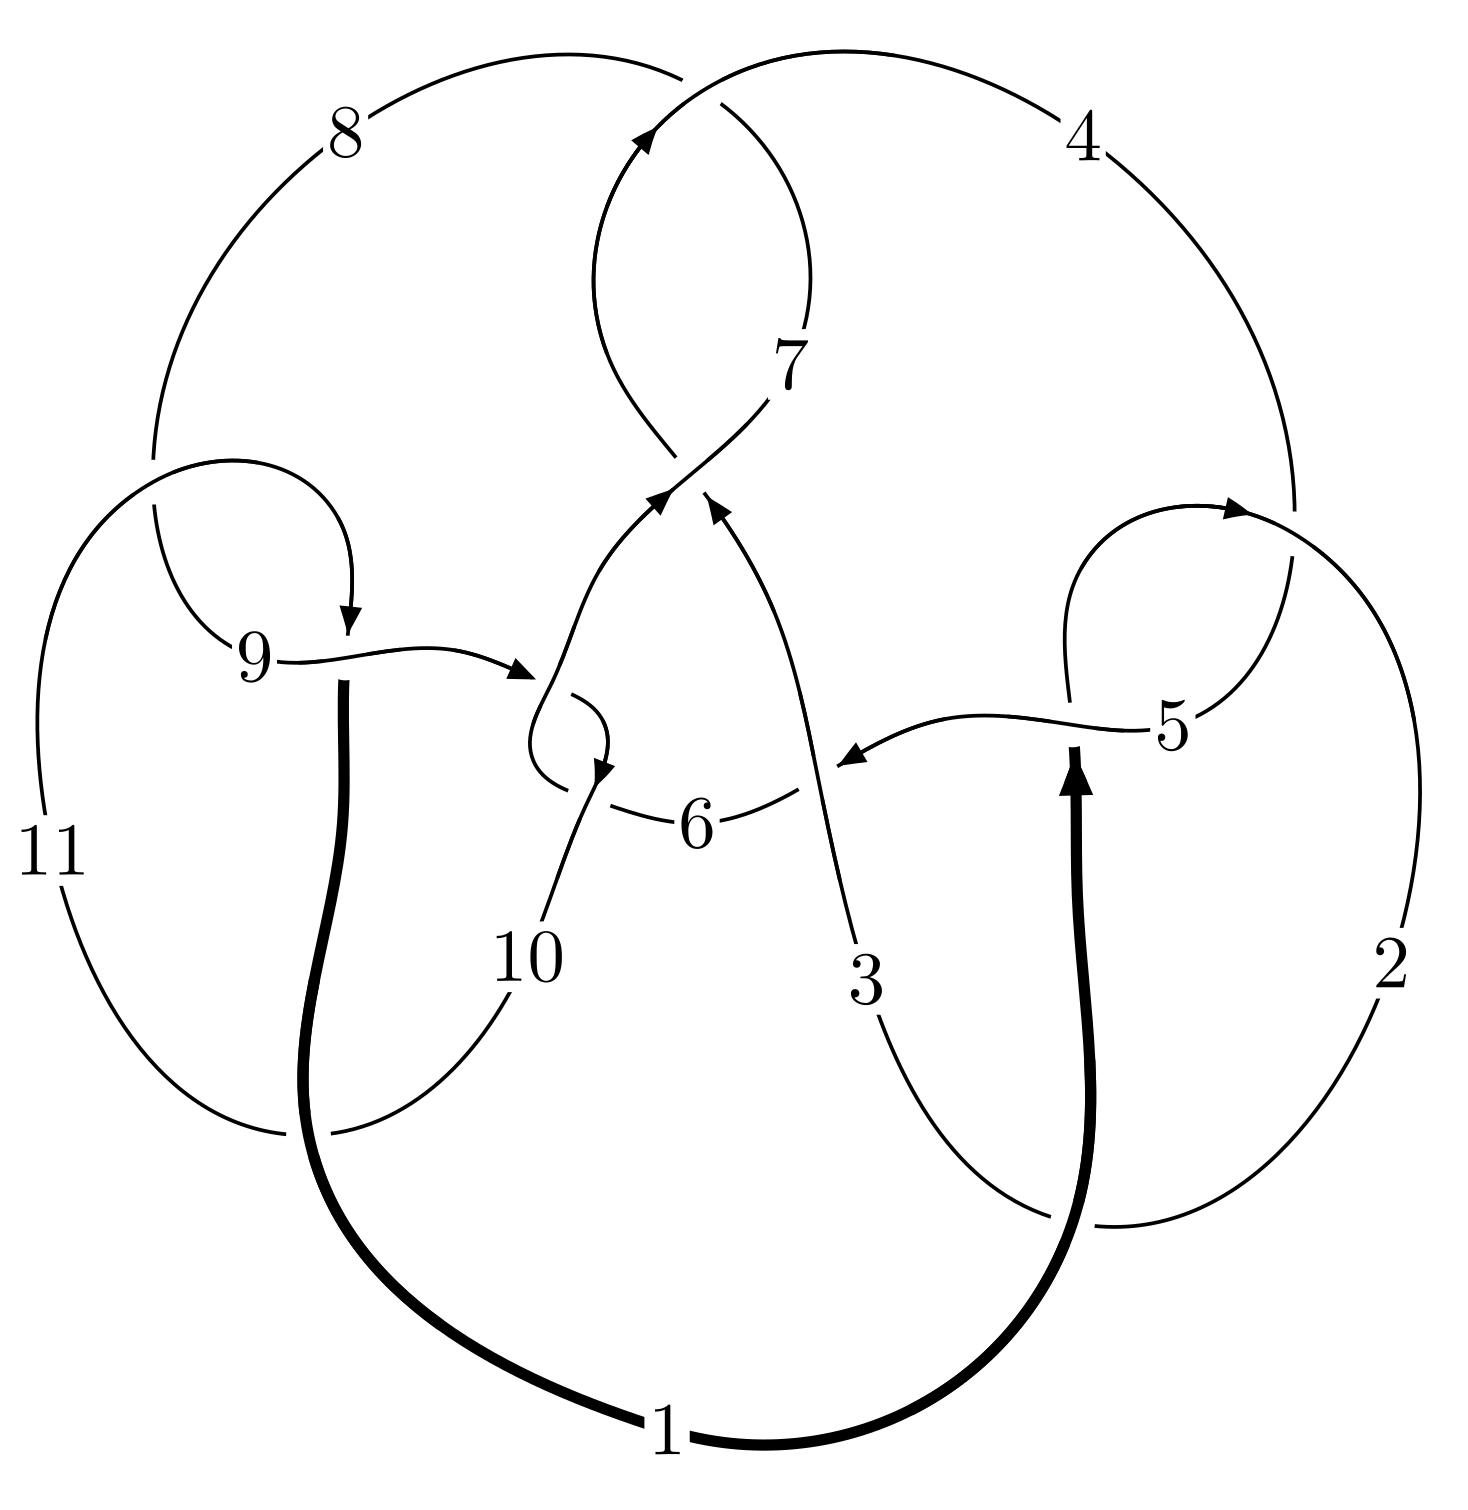
\includegraphics[width=112pt]{../../../GIT/diagram.site/Diagrams/png/622_11n_6.png}\\
\ \ \ A knot diagram\footnotemark}&
\allowdisplaybreaks
\textbf{Linearized knot diagam} \\
\cline{2-2}
 &
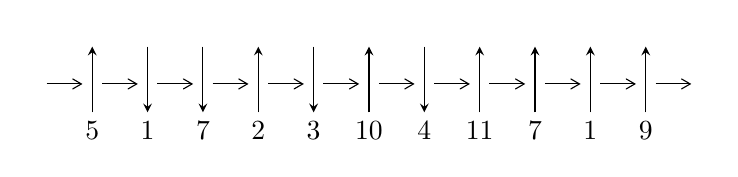
\begin{tikzpicture}[x=20pt, y=17pt]
	% nodes
	\node (C0) at (0, 0) {};
	\node (C1) at (1, 0) {};
	\node (C1U) at (1, +1) {};
	\node (C1D) at (1, -1) {5};

	\node (C2) at (2, 0) {};
	\node (C2U) at (2, +1) {};
	\node (C2D) at (2, -1) {1};

	\node (C3) at (3, 0) {};
	\node (C3U) at (3, +1) {};
	\node (C3D) at (3, -1) {7};

	\node (C4) at (4, 0) {};
	\node (C4U) at (4, +1) {};
	\node (C4D) at (4, -1) {2};

	\node (C5) at (5, 0) {};
	\node (C5U) at (5, +1) {};
	\node (C5D) at (5, -1) {3};

	\node (C6) at (6, 0) {};
	\node (C6U) at (6, +1) {};
	\node (C6D) at (6, -1) {10};

	\node (C7) at (7, 0) {};
	\node (C7U) at (7, +1) {};
	\node (C7D) at (7, -1) {4};

	\node (C8) at (8, 0) {};
	\node (C8U) at (8, +1) {};
	\node (C8D) at (8, -1) {11};

	\node (C9) at (9, 0) {};
	\node (C9U) at (9, +1) {};
	\node (C9D) at (9, -1) {7};

	\node (C10) at (10, 0) {};
	\node (C10U) at (10, +1) {};
	\node (C10D) at (10, -1) {1};

	\node (C11) at (11, 0) {};
	\node (C11U) at (11, +1) {};
	\node (C11D) at (11, -1) {9};
	\node (C12) at (12, 0) {};

	% arrows
	\draw[->,>={angle 60}]
	(C0) edge (C1) (C1) edge (C2) (C2) edge (C3) (C3) edge (C4) (C4) edge (C5) (C5) edge (C6) (C6) edge (C7) (C7) edge (C8) (C8) edge (C9) (C9) edge (C10) (C10) edge (C11) (C11) edge (C12) ;	\draw[->,>=stealth]
	(C1D) edge (C1U) (C2U) edge (C2D) (C3U) edge (C3D) (C4D) edge (C4U) (C5U) edge (C5D) (C6D) edge (C6U) (C7U) edge (C7D) (C8D) edge (C8U) (C9D) edge (C9U) (C10D) edge (C10U) (C11D) edge (C11U) ;
	\end{tikzpicture} \\
\hhline{~~} \\& 
\textbf{Solving Sequence} \\ \cline{2-2} 
 &
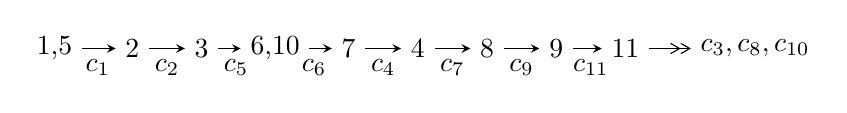
\begin{tikzpicture}[x=25pt, y=7pt]
	% node
	\node (A0) at (-1/8, 0) {1,5};
	\node (A1) at (1, 0) {2};
	\node (A2) at (2, 0) {3};
	\node (A3) at (49/16, 0) {6,10};
	\node (A4) at (33/8, 0) {7};
	\node (A5) at (41/8, 0) {4};
	\node (A6) at (49/8, 0) {8};
	\node (A7) at (57/8, 0) {9};
	\node (A8) at (65/8, 0) {11};
	\node (C1) at (1/2, -1) {$c_{1}$};
	\node (C2) at (3/2, -1) {$c_{2}$};
	\node (C3) at (5/2, -1) {$c_{5}$};
	\node (C4) at (29/8, -1) {$c_{6}$};
	\node (C5) at (37/8, -1) {$c_{4}$};
	\node (C6) at (45/8, -1) {$c_{7}$};
	\node (C7) at (53/8, -1) {$c_{9}$};
	\node (C8) at (61/8, -1) {$c_{11}$};
	\node (A9) at (10, 0) {$c_{3},c_{8},c_{10}$};

	% edge
	\draw[->,>=stealth]	
	(A0) edge (A1) (A1) edge (A2) (A2) edge (A3) (A3) edge (A4) (A4) edge (A5) (A5) edge (A6) (A6) edge (A7) (A7) edge (A8) ;
	\draw[->>,>={angle 60}]	
	(A8) edge (A9);
\end{tikzpicture} \\ 

\end{tabular} \\

\footnotetext{
The image of knot diagram is generated by the software ``\textbf{Draw programme}" developed by Andrew Bartholomew(\url{http://www.layer8.co.uk/maths/draw/index.htm\#Running-draw}), where we modified some parts for our purpose(\url{https://github.com/CATsTAILs/LinksPainter}).
}\phantom \\ \newline 
\centering \textbf{Ideals for irreducible components\footnotemark of $X_{\text{par}}$} 
 
\begin{align*}
I^u_{1}&=\langle 
-4445 u^{18}+25166 u^{17}+\cdots+157228 b-130422,\\
\phantom{I^u_{1}}&\phantom{= \langle  }102053 u^{18}-516382 u^{17}+\cdots+157228 a+1635396,\;u^{19}-5 u^{18}+\cdots+18 u-1\rangle \\
I^u_{2}&=\langle 
3 a^2 u+a^2-4 a u+7 b+a+u-9,\;a^3+a^2 u- a^2+3 a u+2 a-5 u-5,\;u^2+u+1\rangle \\
I^u_{3}&=\langle 
b-1,\;u^4- u^3+2 u^2+a- u+1,\;u^5- u^4+2 u^3- u^2+u-1\rangle \\
\\
\end{align*}
\raggedright * 3 irreducible components of $\dim_{\mathbb{C}}=0$, with total 30 representations.\\
\footnotetext{All coefficients of polynomials are rational numbers. But the coefficients are sometimes approximated in decimal forms when there is not enough margin.}
\newpage
\renewcommand{\arraystretch}{1}
\centering \section*{I. $I^u_{1}= \langle -4445 u^{18}+2.52\times10^{4} u^{17}+\cdots+1.57\times10^{5} b-1.30\times10^{5},\;1.02\times10^{5} u^{18}-5.16\times10^{5} u^{17}+\cdots+1.57\times10^{5} a+1.64\times10^{6},\;u^{19}-5 u^{18}+\cdots+18 u-1 \rangle$}
\flushleft \textbf{(i) Arc colorings}\\
\begin{tabular}{m{7pt} m{180pt} m{7pt} m{180pt} }
\flushright $a_{1}=$&$\begin{pmatrix}1\\0\end{pmatrix}$ \\
\flushright $a_{5}=$&$\begin{pmatrix}0\\u\end{pmatrix}$ \\
\flushright $a_{2}=$&$\begin{pmatrix}1\\- u^2\end{pmatrix}$ \\
\flushright $a_{3}=$&$\begin{pmatrix}u^2+1\\- u^2\end{pmatrix}$ \\
\flushright $a_{6}=$&$\begin{pmatrix}- u^5-2 u^3- u\\u^5+u^3+u\end{pmatrix}$ \\
\flushright $a_{10}=$&$\begin{pmatrix}-0.649077 u^{18}+3.28429 u^{17}+\cdots+38.5711 u-10.4014\\0.0282710 u^{18}-0.160061 u^{17}+\cdots-2.36210 u+0.829509\end{pmatrix}$ \\
\flushright $a_{7}=$&$\begin{pmatrix}0.638684 u^{18}-2.98006 u^{17}+\cdots-23.7743 u+5.48846\\-0.213359 u^{18}+1.10318 u^{17}+\cdots+6.00785 u-0.638684\end{pmatrix}$ \\
\flushright $a_{4}=$&$\begin{pmatrix}- u\\u^3+u\end{pmatrix}$ \\
\flushright $a_{8}=$&$\begin{pmatrix}0.586798 u^{18}-2.76808 u^{17}+\cdots-23.8489 u+5.47099\\-0.195678 u^{18}+0.900151 u^{17}+\cdots+5.28026 u-0.573772\end{pmatrix}$ \\
\flushright $a_{9}=$&$\begin{pmatrix}-0.987191 u^{18}+4.82270 u^{17}+\cdots+47.6110 u-13.0026\\0.180432 u^{18}-0.834985 u^{17}+\cdots-5.84697 u+1.16762\end{pmatrix}$ \\
\flushright $a_{11}=$&$\begin{pmatrix}-0.620805 u^{18}+3.12423 u^{17}+\cdots+36.2090 u-9.57192\\0.0282710 u^{18}-0.160061 u^{17}+\cdots-2.36210 u+0.829509\end{pmatrix}$\\ \flushright $a_{11}=$&$\begin{pmatrix}-0.620805 u^{18}+3.12423 u^{17}+\cdots+36.2090 u-9.57192\\0.0282710 u^{18}-0.160061 u^{17}+\cdots-2.36210 u+0.829509\end{pmatrix}$\\&\end{tabular}
\flushleft \textbf{(ii) Obstruction class $= -1$}\\~\\
\flushleft \textbf{(iii) Cusp Shapes $= \frac{48467}{78614} u^{18}-\frac{220275}{78614} u^{17}+\cdots-\frac{2697747}{78614} u+\frac{420630}{39307}$}\\~\\
\newpage\renewcommand{\arraystretch}{1}
\flushleft \textbf{(iv) u-Polynomials at the component}\newline \\
\begin{tabular}{m{50pt}|m{274pt}}
Crossings & \hspace{64pt}u-Polynomials at each crossing \\
\hline $$\begin{aligned}c_{1},c_{4}\end{aligned}$$&$\begin{aligned}
&u^{19}+5 u^{18}+\cdots+18 u+1
\end{aligned}$\\
\hline $$\begin{aligned}c_{2}\end{aligned}$$&$\begin{aligned}
&u^{19}+15 u^{18}+\cdots+208 u-1
\end{aligned}$\\
\hline $$\begin{aligned}c_{3},c_{7}\end{aligned}$$&$\begin{aligned}
&u^{19}+2 u^{18}+\cdots+96 u-64
\end{aligned}$\\
\hline $$\begin{aligned}c_{5}\end{aligned}$$&$\begin{aligned}
&u^{19}-5 u^{18}+\cdots+854 u+49
\end{aligned}$\\
\hline $$\begin{aligned}c_{6},c_{9}\end{aligned}$$&$\begin{aligned}
&u^{19}+3 u^{18}+\cdots-88 u^2-32
\end{aligned}$\\
\hline $$\begin{aligned}c_{8},c_{11}\end{aligned}$$&$\begin{aligned}
&u^{19}+8 u^{18}+\cdots-15 u-1
\end{aligned}$\\
\hline $$\begin{aligned}c_{10}\end{aligned}$$&$\begin{aligned}
&u^{19}+2 u^{18}+\cdots+69 u-1
\end{aligned}$\\
\hline
\end{tabular}\\~\\
\newpage\renewcommand{\arraystretch}{1}
\flushleft \textbf{(v) Riley Polynomials at the component}\newline \\
\begin{tabular}{m{50pt}|m{274pt}}
Crossings & \hspace{64pt}Riley Polynomials at each crossing \\
\hline $$\begin{aligned}c_{1},c_{4}\end{aligned}$$&$\begin{aligned}
&y^{19}+15 y^{18}+\cdots+208 y-1
\end{aligned}$\\
\hline $$\begin{aligned}c_{2}\end{aligned}$$&$\begin{aligned}
&y^{19}-17 y^{18}+\cdots+45036 y-1
\end{aligned}$\\
\hline $$\begin{aligned}c_{3},c_{7}\end{aligned}$$&$\begin{aligned}
&y^{19}-40 y^{18}+\cdots+17408 y-4096
\end{aligned}$\\
\hline $$\begin{aligned}c_{5}\end{aligned}$$&$\begin{aligned}
&y^{19}-49 y^{18}+\cdots+501760 y-2401
\end{aligned}$\\
\hline $$\begin{aligned}c_{6},c_{9}\end{aligned}$$&$\begin{aligned}
&y^{19}+39 y^{18}+\cdots-5632 y-1024
\end{aligned}$\\
\hline $$\begin{aligned}c_{8},c_{11}\end{aligned}$$&$\begin{aligned}
&y^{19}+2 y^{18}+\cdots+69 y-1
\end{aligned}$\\
\hline $$\begin{aligned}c_{10}\end{aligned}$$&$\begin{aligned}
&y^{19}+54 y^{18}+\cdots-2699 y-1
\end{aligned}$\\
\hline
\end{tabular}\\~\\
\newpage\flushleft \textbf{(vi) Complex Volumes and Cusp Shapes}
$$\begin{array}{c|c|c}  
\text{Solutions to }I^u_{1}& \I (\text{vol} + \sqrt{-1}CS) & \text{Cusp shape}\\
 \hline 
\begin{aligned}
u &= -0.459827 + 0.896977 I \\
a &= \phantom{-}2.21570 + 0.93164 I \\
b &= \phantom{-}0.888580 + 0.149996 I\end{aligned}
 & \phantom{-}1.34528 - 1.87445 I & \phantom{-}29.9213 + 13.6703 I \\ \hline\begin{aligned}
u &= -0.459827 - 0.896977 I \\
a &= \phantom{-}2.21570 - 0.93164 I \\
b &= \phantom{-}0.888580 - 0.149996 I\end{aligned}
 & \phantom{-}1.34528 + 1.87445 I & \phantom{-}29.9213 - 13.6703 I \\ \hline\begin{aligned}
u &= -0.351109 + 0.745933 I \\
a &= \phantom{-}0.875169 - 0.043573 I \\
b &= \phantom{-}0.0093474 + 0.0139592 I\end{aligned}
 & -0.22305 - 1.43330 I & -1.61645 + 4.92513 I \\ \hline\begin{aligned}
u &= -0.351109 - 0.745933 I \\
a &= \phantom{-}0.875169 + 0.043573 I \\
b &= \phantom{-}0.0093474 - 0.0139592 I\end{aligned}
 & -0.22305 + 1.43330 I & -1.61645 - 4.92513 I \\ \hline\begin{aligned}
u &= \phantom{-}0.389305 + 1.111150 I \\
a &= -0.862837 - 0.197630 I \\
b &= \phantom{-}0.668732 + 0.907469 I\end{aligned}
 & -4.23087 + 5.58158 I & -3.54918 - 7.60584 I \\ \hline\begin{aligned}
u &= \phantom{-}0.389305 - 1.111150 I \\
a &= -0.862837 + 0.197630 I \\
b &= \phantom{-}0.668732 - 0.907469 I\end{aligned}
 & -4.23087 - 5.58158 I & -3.54918 + 7.60584 I \\ \hline\begin{aligned}
u &= -0.265172 + 1.190510 I \\
a &= \phantom{-}0.759357 + 0.604707 I \\
b &= -0.460697 + 0.797639 I\end{aligned}
 & -1.40496 - 0.89543 I & -0.827466 + 0.267848 I \\ \hline\begin{aligned}
u &= -0.265172 - 1.190510 I \\
a &= \phantom{-}0.759357 - 0.604707 I \\
b &= -0.460697 - 0.797639 I\end{aligned}
 & -1.40496 + 0.89543 I & -0.827466 - 0.267848 I \\ \hline\begin{aligned}
u &= \phantom{-}1.236570 + 0.125353 I \\
a &= -0.08471 + 3.83451 I \\
b &= \phantom{-}0.07758 - 3.21706 I\end{aligned}
 & -14.6816 - 4.7277 I & \phantom{-}1.60029 + 1.79597 I \\ \hline\begin{aligned}
u &= \phantom{-}1.236570 - 0.125353 I \\
a &= -0.08471 - 3.83451 I \\
b &= \phantom{-}0.07758 + 3.21706 I\end{aligned}
 & -14.6816 + 4.7277 I & \phantom{-}1.60029 - 1.79597 I\\
 \hline 
 \end{array}$$\newpage$$\begin{array}{c|c|c}  
\text{Solutions to }I^u_{1}& \I (\text{vol} + \sqrt{-1}CS) & \text{Cusp shape}\\
 \hline 
\begin{aligned}
u &= \phantom{-}0.578208 + 0.363922 I \\
a &= \phantom{-}1.06872 + 1.66313 I \\
b &= -0.039673 - 0.833778 I\end{aligned}
 & -2.02190 - 1.85032 I & \phantom{-}0.40467 + 3.82422 I \\ \hline\begin{aligned}
u &= \phantom{-}0.578208 - 0.363922 I \\
a &= \phantom{-}1.06872 - 1.66313 I \\
b &= -0.039673 + 0.833778 I\end{aligned}
 & -2.02190 + 1.85032 I & \phantom{-}0.40467 - 3.82422 I \\ \hline\begin{aligned}
u &= \phantom{-}0.12128 + 1.49762 I \\
a &= \phantom{-}1.41899 + 0.08782 I \\
b &= -2.23717 - 0.89116 I\end{aligned}
 & -8.30737 + 0.41800 I & -1.92088 - 0.17258 I \\ \hline\begin{aligned}
u &= \phantom{-}0.12128 - 1.49762 I \\
a &= \phantom{-}1.41899 - 0.08782 I \\
b &= -2.23717 + 0.89116 I\end{aligned}
 & -8.30737 - 0.41800 I & -1.92088 + 0.17258 I \\ \hline\begin{aligned}
u &= \phantom{-}0.66518 + 1.37702 I \\
a &= -2.46188 - 1.46194 I \\
b &= \phantom{-}0.83728 + 3.06795 I\end{aligned}
 & -18.5579 + 11.4070 I & \phantom{-}0.02962 - 4.80086 I \\ \hline\begin{aligned}
u &= \phantom{-}0.66518 - 1.37702 I \\
a &= -2.46188 + 1.46194 I \\
b &= \phantom{-}0.83728 - 3.06795 I\end{aligned}
 & -18.5579 - 11.4070 I & \phantom{-}0.02962 + 4.80086 I \\ \hline\begin{aligned}
u &= \phantom{-}0.55124 + 1.54379 I \\
a &= \phantom{-}2.12819 + 1.66552 I \\
b &= -1.08511 - 3.58320 I\end{aligned}
 & \phantom{-}19.5193 + 1.7269 I & -0.878629 - 0.706920 I \\ \hline\begin{aligned}
u &= \phantom{-}0.55124 - 1.54379 I \\
a &= \phantom{-}2.12819 - 1.66552 I \\
b &= -1.08511 + 3.58320 I\end{aligned}
 & \phantom{-}19.5193 - 1.7269 I & -0.878629 + 0.706920 I \\ \hline\begin{aligned}
u &= \phantom{-}0.0686432\phantom{ +0.000000I} \\
a &= -8.11341\phantom{ +0.000000I} \\
b &= \phantom{-}0.682273\phantom{ +0.000000I}\end{aligned}
 & \phantom{-}1.19847\phantom{ +0.000000I} & \phantom{-}8.67340\phantom{ +0.000000I}\\
 \hline 
 \end{array}$$\newpage\newpage\renewcommand{\arraystretch}{1}
\centering \section*{II. $I^u_{2}= \langle 3 a^2 u+a^2-4 a u+7 b+a+u-9,\;a^3+a^2 u- a^2+3 a u+2 a-5 u-5,\;u^2+u+1 \rangle$}
\flushleft \textbf{(i) Arc colorings}\\
\begin{tabular}{m{7pt} m{180pt} m{7pt} m{180pt} }
\flushright $a_{1}=$&$\begin{pmatrix}1\\0\end{pmatrix}$ \\
\flushright $a_{5}=$&$\begin{pmatrix}0\\u\end{pmatrix}$ \\
\flushright $a_{2}=$&$\begin{pmatrix}1\\u+1\end{pmatrix}$ \\
\flushright $a_{3}=$&$\begin{pmatrix}- u\\u+1\end{pmatrix}$ \\
\flushright $a_{6}=$&$\begin{pmatrix}-1\\0\end{pmatrix}$ \\
\flushright $a_{10}=$&$\begin{pmatrix}a\\-\frac{3}{7} a^2 u+\frac{4}{7} a u+\cdots-\frac{1}{7} a+\frac{9}{7}\end{pmatrix}$ \\
\flushright $a_{7}=$&$\begin{pmatrix}-\frac{1}{7} a^2 u-\frac{1}{7} a u+\cdots+\frac{2}{7} a+\frac{3}{7}\\-\frac{4}{7} a^2 u+\frac{3}{7} a u+\cdots+\frac{1}{7} a+\frac{5}{7}\end{pmatrix}$ \\
\flushright $a_{4}=$&$\begin{pmatrix}- u\\u+1\end{pmatrix}$ \\
\flushright $a_{8}=$&$\begin{pmatrix}-\frac{1}{7} a^2 u-\frac{1}{7} a u+\cdots+\frac{2}{7} a+\frac{3}{7}\\-\frac{4}{7} a^2 u+\frac{3}{7} a u+\cdots+\frac{1}{7} a+\frac{5}{7}\end{pmatrix}$ \\
\flushright $a_{9}=$&$\begin{pmatrix}-\frac{3}{7} a^2 u-\frac{3}{7} a u+\cdots-\frac{1}{7} a+\frac{16}{7}\\-\frac{1}{7} a^2 u-\frac{1}{7} a u+\cdots+\frac{2}{7} a+\frac{3}{7}\end{pmatrix}$ \\
\flushright $a_{11}=$&$\begin{pmatrix}-\frac{3}{7} a^2 u+\frac{4}{7} a u+\cdots+\frac{6}{7} a+\frac{9}{7}\\-\frac{3}{7} a^2 u+\frac{4}{7} a u+\cdots-\frac{1}{7} a+\frac{9}{7}\end{pmatrix}$\\ \flushright $a_{11}=$&$\begin{pmatrix}-\frac{3}{7} a^2 u+\frac{4}{7} a u+\cdots+\frac{6}{7} a+\frac{9}{7}\\-\frac{3}{7} a^2 u+\frac{4}{7} a u+\cdots-\frac{1}{7} a+\frac{9}{7}\end{pmatrix}$\\&\end{tabular}
\flushleft \textbf{(ii) Obstruction class $= 1$}\\~\\
\flushleft \textbf{(iii) Cusp Shapes $= \frac{17}{7} a^2 u+\frac{29}{7} a^2-\frac{4}{7} a u-\frac{6}{7} a+\frac{99}{7} u+\frac{12}{7}$}\\~\\
\newpage\renewcommand{\arraystretch}{1}
\flushleft \textbf{(iv) u-Polynomials at the component}\newline \\
\begin{tabular}{m{50pt}|m{274pt}}
Crossings & \hspace{64pt}u-Polynomials at each crossing \\
\hline $$\begin{aligned}c_{1},c_{2},c_{5}\end{aligned}$$&$\begin{aligned}
&(u^2+u+1)^3
\end{aligned}$\\
\hline $$\begin{aligned}c_{3},c_{7}\end{aligned}$$&$\begin{aligned}
&u^6
\end{aligned}$\\
\hline $$\begin{aligned}c_{4}\end{aligned}$$&$\begin{aligned}
&(u^2- u+1)^3
\end{aligned}$\\
\hline $$\begin{aligned}c_{6},c_{10}\end{aligned}$$&$\begin{aligned}
&(u^3+u^2+2 u+1)^2
\end{aligned}$\\
\hline $$\begin{aligned}c_{8}\end{aligned}$$&$\begin{aligned}
&(u^3- u^2+1)^2
\end{aligned}$\\
\hline $$\begin{aligned}c_{9}\end{aligned}$$&$\begin{aligned}
&(u^3- u^2+2 u-1)^2
\end{aligned}$\\
\hline $$\begin{aligned}c_{11}\end{aligned}$$&$\begin{aligned}
&(u^3+u^2-1)^2
\end{aligned}$\\
\hline
\end{tabular}\\~\\
\newpage\renewcommand{\arraystretch}{1}
\flushleft \textbf{(v) Riley Polynomials at the component}\newline \\
\begin{tabular}{m{50pt}|m{274pt}}
Crossings & \hspace{64pt}Riley Polynomials at each crossing \\
\hline $$\begin{aligned}c_{1},c_{2},c_{4}\\c_{5}\end{aligned}$$&$\begin{aligned}
&(y^2+y+1)^3
\end{aligned}$\\
\hline $$\begin{aligned}c_{3},c_{7}\end{aligned}$$&$\begin{aligned}
&y^6
\end{aligned}$\\
\hline $$\begin{aligned}c_{6},c_{9},c_{10}\end{aligned}$$&$\begin{aligned}
&(y^3+3 y^2+2 y-1)^2
\end{aligned}$\\
\hline $$\begin{aligned}c_{8},c_{11}\end{aligned}$$&$\begin{aligned}
&(y^3- y^2+2 y-1)^2
\end{aligned}$\\
\hline
\end{tabular}\\~\\
\newpage\flushleft \textbf{(vi) Complex Volumes and Cusp Shapes}
$$\begin{array}{c|c|c}  
\text{Solutions to }I^u_{2}& \I (\text{vol} + \sqrt{-1}CS) & \text{Cusp shape}\\
 \hline 
\begin{aligned}
u &= -0.500000 + 0.866025 I \\
a &= \phantom{-}1.46996 - 0.49350 I \\
b &= \phantom{-}0.569840\phantom{ +0.000000I}\end{aligned}
 & \phantom{-}1.11345 - 2.02988 I & \phantom{-}2.22484 + 11.58609 I \\ \hline\begin{aligned}
u &= -0.500000 + 0.866025 I \\
a &= -1.11700 + 1.21217 I \\
b &= \phantom{-}0.215080 - 1.307140 I\end{aligned}
 & -3.02413 - 4.85801 I & \phantom{-}0.92725 + 3.71146 I \\ \hline\begin{aligned}
u &= -0.500000 + 0.866025 I \\
a &= \phantom{-}1.14704 - 1.58470 I \\
b &= \phantom{-}0.215080 + 1.307140 I\end{aligned}
 & -3.02413 + 0.79824 I & -2.65209 - 0.57512 I \\ \hline\begin{aligned}
u &= -0.500000 - 0.866025 I \\
a &= \phantom{-}1.46996 + 0.49350 I \\
b &= \phantom{-}0.569840\phantom{ +0.000000I}\end{aligned}
 & \phantom{-}1.11345 + 2.02988 I & \phantom{-}2.22484 - 11.58609 I \\ \hline\begin{aligned}
u &= -0.500000 - 0.866025 I \\
a &= -1.11700 - 1.21217 I \\
b &= \phantom{-}0.215080 + 1.307140 I\end{aligned}
 & -3.02413 + 4.85801 I & \phantom{-}0.92725 - 3.71146 I \\ \hline\begin{aligned}
u &= -0.500000 - 0.866025 I \\
a &= \phantom{-}1.14704 + 1.58470 I \\
b &= \phantom{-}0.215080 - 1.307140 I\end{aligned}
 & -3.02413 - 0.79824 I & -2.65209 + 0.57512 I\\
 \hline 
 \end{array}$$\newpage\newpage\renewcommand{\arraystretch}{1}
\centering \section*{III. $I^u_{3}= \langle b-1,\;u^4- u^3+2 u^2+a- u+1,\;u^5- u^4+2 u^3- u^2+u-1 \rangle$}
\flushleft \textbf{(i) Arc colorings}\\
\begin{tabular}{m{7pt} m{180pt} m{7pt} m{180pt} }
\flushright $a_{1}=$&$\begin{pmatrix}1\\0\end{pmatrix}$ \\
\flushright $a_{5}=$&$\begin{pmatrix}0\\u\end{pmatrix}$ \\
\flushright $a_{2}=$&$\begin{pmatrix}1\\- u^2\end{pmatrix}$ \\
\flushright $a_{3}=$&$\begin{pmatrix}u^2+1\\- u^2\end{pmatrix}$ \\
\flushright $a_{6}=$&$\begin{pmatrix}- u^4- u^2-1\\u^4- u^3+u^2+1\end{pmatrix}$ \\
\flushright $a_{10}=$&$\begin{pmatrix}- u^4+u^3-2 u^2+u-1\\1\end{pmatrix}$ \\
\flushright $a_{7}=$&$\begin{pmatrix}- u^4- u^2-1\\u^4- u^3+u^2+1\end{pmatrix}$ \\
\flushright $a_{4}=$&$\begin{pmatrix}- u\\u^3+u\end{pmatrix}$ \\
\flushright $a_{8}=$&$\begin{pmatrix}-1\\0\end{pmatrix}$ \\
\flushright $a_{9}=$&$\begin{pmatrix}- u^4+u^3-2 u^2+u-1\\1\end{pmatrix}$ \\
\flushright $a_{11}=$&$\begin{pmatrix}- u^4+u^3-2 u^2+u\\1\end{pmatrix}$\\ \flushright $a_{11}=$&$\begin{pmatrix}- u^4+u^3-2 u^2+u\\1\end{pmatrix}$\\&\end{tabular}
\flushleft \textbf{(ii) Obstruction class $= 1$}\\~\\
\flushleft \textbf{(iii) Cusp Shapes $= -3 u^4+5 u^3-4 u^2+3$}\\~\\
\newpage\renewcommand{\arraystretch}{1}
\flushleft \textbf{(iv) u-Polynomials at the component}\newline \\
\begin{tabular}{m{50pt}|m{274pt}}
Crossings & \hspace{64pt}u-Polynomials at each crossing \\
\hline $$\begin{aligned}c_{1}\end{aligned}$$&$\begin{aligned}
&u^5- u^4+2 u^3- u^2+u-1
\end{aligned}$\\
\hline $$\begin{aligned}c_{2}\end{aligned}$$&$\begin{aligned}
&u^5+3 u^4+4 u^3+u^2- u-1
\end{aligned}$\\
\hline $$\begin{aligned}c_{3}\end{aligned}$$&$\begin{aligned}
&u^5+u^4-2 u^3- u^2+u-1
\end{aligned}$\\
\hline $$\begin{aligned}c_{4}\end{aligned}$$&$\begin{aligned}
&u^5+u^4+2 u^3+u^2+u+1
\end{aligned}$\\
\hline $$\begin{aligned}c_{5},c_{7}\end{aligned}$$&$\begin{aligned}
&u^5- u^4-2 u^3+u^2+u+1
\end{aligned}$\\
\hline $$\begin{aligned}c_{6},c_{9}\end{aligned}$$&$\begin{aligned}
&u^5
\end{aligned}$\\
\hline $$\begin{aligned}c_{8},c_{10}\end{aligned}$$&$\begin{aligned}
&(u+1)^5
\end{aligned}$\\
\hline $$\begin{aligned}c_{11}\end{aligned}$$&$\begin{aligned}
&(u-1)^5
\end{aligned}$\\
\hline
\end{tabular}\\~\\
\newpage\renewcommand{\arraystretch}{1}
\flushleft \textbf{(v) Riley Polynomials at the component}\newline \\
\begin{tabular}{m{50pt}|m{274pt}}
Crossings & \hspace{64pt}Riley Polynomials at each crossing \\
\hline $$\begin{aligned}c_{1},c_{4}\end{aligned}$$&$\begin{aligned}
&y^5+3 y^4+4 y^3+y^2- y-1
\end{aligned}$\\
\hline $$\begin{aligned}c_{2}\end{aligned}$$&$\begin{aligned}
&y^5- y^4+8 y^3-3 y^2+3 y-1
\end{aligned}$\\
\hline $$\begin{aligned}c_{3},c_{5},c_{7}\end{aligned}$$&$\begin{aligned}
&y^5-5 y^4+8 y^3-3 y^2- y-1
\end{aligned}$\\
\hline $$\begin{aligned}c_{6},c_{9}\end{aligned}$$&$\begin{aligned}
&y^5
\end{aligned}$\\
\hline $$\begin{aligned}c_{8},c_{10},c_{11}\end{aligned}$$&$\begin{aligned}
&(y-1)^5
\end{aligned}$\\
\hline
\end{tabular}\\~\\
\newpage\flushleft \textbf{(vi) Complex Volumes and Cusp Shapes}
$$\begin{array}{c|c|c}  
\text{Solutions to }I^u_{3}& \I (\text{vol} + \sqrt{-1}CS) & \text{Cusp shape}\\
 \hline 
\begin{aligned}
u &= -0.339110 + 0.822375 I \\
a &= \phantom{-}0.428550 + 1.039280 I \\
b &= \phantom{-}1.00000\phantom{ +0.000000I}\end{aligned}
 & \phantom{-}1.31583 - 1.53058 I & \phantom{-}8.47842 - 1.00973 I \\ \hline\begin{aligned}
u &= -0.339110 - 0.822375 I \\
a &= \phantom{-}0.428550 - 1.039280 I \\
b &= \phantom{-}1.00000\phantom{ +0.000000I}\end{aligned}
 & \phantom{-}1.31583 + 1.53058 I & \phantom{-}8.47842 + 1.00973 I \\ \hline\begin{aligned}
u &= \phantom{-}0.766826\phantom{ +0.000000I} \\
a &= -1.30408\phantom{ +0.000000I} \\
b &= \phantom{-}1.00000\phantom{ +0.000000I}\end{aligned}
 & -0.756147\phantom{ +0.000000I} & \phantom{-}1.86520\phantom{ +0.000000I} \\ \hline\begin{aligned}
u &= \phantom{-}0.455697 + 1.200150 I \\
a &= -0.276511 + 0.728237 I \\
b &= \phantom{-}1.00000\phantom{ +0.000000I}\end{aligned}
 & -4.22763 + 4.40083 I & -2.41100 - 1.19010 I \\ \hline\begin{aligned}
u &= \phantom{-}0.455697 - 1.200150 I \\
a &= -0.276511 - 0.728237 I \\
b &= \phantom{-}1.00000\phantom{ +0.000000I}\end{aligned}
 & -4.22763 - 4.40083 I & -2.41100 + 1.19010 I\\
 \hline 
 \end{array}$$\newpage
\newpage\renewcommand{\arraystretch}{1}
\centering \section*{ IV. u-Polynomials}
\begin{tabular}{m{50pt}|m{274pt}}
Crossings & \hspace{64pt}u-Polynomials at each crossing \\
\hline $$\begin{aligned}c_{1}\end{aligned}$$&$\begin{aligned}
&((u^2+u+1)^3)(u^5- u^4+\cdots+u-1)(u^{19}+5 u^{18}+\cdots+18 u+1)
\end{aligned}$\\
\hline $$\begin{aligned}c_{2}\end{aligned}$$&$\begin{aligned}
&(u^2+u+1)^3(u^5+3 u^4+4 u^3+u^2- u-1)\\
&\cdot(u^{19}+15 u^{18}+\cdots+208 u-1)
\end{aligned}$\\
\hline $$\begin{aligned}c_{3}\end{aligned}$$&$\begin{aligned}
&u^6(u^5+u^4+\cdots+u-1)(u^{19}+2 u^{18}+\cdots+96 u-64)
\end{aligned}$\\
\hline $$\begin{aligned}c_{4}\end{aligned}$$&$\begin{aligned}
&((u^2- u+1)^3)(u^5+u^4+\cdots+u+1)(u^{19}+5 u^{18}+\cdots+18 u+1)
\end{aligned}$\\
\hline $$\begin{aligned}c_{5}\end{aligned}$$&$\begin{aligned}
&((u^2+u+1)^3)(u^5- u^4+\cdots+u+1)(u^{19}-5 u^{18}+\cdots+854 u+49)
\end{aligned}$\\
\hline $$\begin{aligned}c_{6}\end{aligned}$$&$\begin{aligned}
&u^5(u^3+u^2+2 u+1)^2(u^{19}+3 u^{18}+\cdots-88 u^2-32)
\end{aligned}$\\
\hline $$\begin{aligned}c_{7}\end{aligned}$$&$\begin{aligned}
&u^6(u^5- u^4+\cdots+u+1)(u^{19}+2 u^{18}+\cdots+96 u-64)
\end{aligned}$\\
\hline $$\begin{aligned}c_{8}\end{aligned}$$&$\begin{aligned}
&((u+1)^5)(u^3- u^2+1)^2(u^{19}+8 u^{18}+\cdots-15 u-1)
\end{aligned}$\\
\hline $$\begin{aligned}c_{9}\end{aligned}$$&$\begin{aligned}
&u^5(u^3- u^2+2 u-1)^2(u^{19}+3 u^{18}+\cdots-88 u^2-32)
\end{aligned}$\\
\hline $$\begin{aligned}c_{10}\end{aligned}$$&$\begin{aligned}
&((u+1)^5)(u^3+u^2+2 u+1)^2(u^{19}+2 u^{18}+\cdots+69 u-1)
\end{aligned}$\\
\hline $$\begin{aligned}c_{11}\end{aligned}$$&$\begin{aligned}
&((u-1)^5)(u^3+u^2-1)^2(u^{19}+8 u^{18}+\cdots-15 u-1)
\end{aligned}$\\
\hline
\end{tabular}\newpage\renewcommand{\arraystretch}{1}
\centering \section*{ V. Riley Polynomials}
\begin{tabular}{m{50pt}|m{274pt}}
Crossings & \hspace{64pt}Riley Polynomials at each crossing \\
\hline $$\begin{aligned}c_{1},c_{4}\end{aligned}$$&$\begin{aligned}
&(y^2+y+1)^3(y^5+3 y^4+4 y^3+y^2- y-1)\\
&\cdot(y^{19}+15 y^{18}+\cdots+208 y-1)
\end{aligned}$\\
\hline $$\begin{aligned}c_{2}\end{aligned}$$&$\begin{aligned}
&(y^2+y+1)^3(y^5- y^4+8 y^3-3 y^2+3 y-1)\\
&\cdot(y^{19}-17 y^{18}+\cdots+45036 y-1)
\end{aligned}$\\
\hline $$\begin{aligned}c_{3},c_{7}\end{aligned}$$&$\begin{aligned}
&y^6(y^5-5 y^4+\cdots- y-1)(y^{19}-40 y^{18}+\cdots+17408 y-4096)
\end{aligned}$\\
\hline $$\begin{aligned}c_{5}\end{aligned}$$&$\begin{aligned}
&(y^2+y+1)^3(y^5-5 y^4+8 y^3-3 y^2- y-1)\\
&\cdot(y^{19}-49 y^{18}+\cdots+501760 y-2401)
\end{aligned}$\\
\hline $$\begin{aligned}c_{6},c_{9}\end{aligned}$$&$\begin{aligned}
&y^5(y^3+3 y^2+2 y-1)^2(y^{19}+39 y^{18}+\cdots-5632 y-1024)
\end{aligned}$\\
\hline $$\begin{aligned}c_{8},c_{11}\end{aligned}$$&$\begin{aligned}
&((y-1)^5)(y^3- y^2+2 y-1)^2(y^{19}+2 y^{18}+\cdots+69 y-1)
\end{aligned}$\\
\hline $$\begin{aligned}c_{10}\end{aligned}$$&$\begin{aligned}
&((y-1)^5)(y^3+3 y^2+2 y-1)^2(y^{19}+54 y^{18}+\cdots-2699 y-1)
\end{aligned}$\\
\hline
\end{tabular}
\vskip 2pc
\end{document}